

%-------------------------------------------------------------------------------
% Dokumenten Klasse
\documentclass[
	final,
	a4paper,
	oneside,
	parskip=full,
	headings=standardclasses,
	headings=big,
	pointednumbers
]{scrartcl}

%-------------------------------------------------------------------------------
% Packete nutzen
\usepackage{ngerman,palatino,setspace}
\usepackage[T1]{fontenc}
\usepackage[latin9]{inputenc}
\usepackage[left=25mm,
            right=25mm,
            top=25mm,
            bottom=25mm]{geometry}
\usepackage{graphicx}
\usepackage[figuresright]{rotating}
\usepackage{scrpage2}
\usepackage{listings}
\usepackage[usenames,dvipsnames,svgnames]{xcolor}
\usepackage[hidelinks]{hyperref}
\usepackage{amsmath}
\usepackage{caption}

%-------------------------------------------------------------------------------
% Kopf- und Fusszeile

%\setlength{\voffset}{-10mm}
%\setlength{\headsep}{0mm}
%\setlength{\topmargin}{5mm}

\pagestyle{scrheadings}
\clearscrheadfoot
\chead{Lineare Transformation von Funktionen}
\cfoot[Seite \thepage]{Seite \thepage}


%-------------------------------------------------------------------------------
% Dokumenten Einstellungen

%-------------------------------------------------------------------------------
% Dokument
\begin{document}
	\begin{sidewaysfigure}
		\centering
		\fbox{
			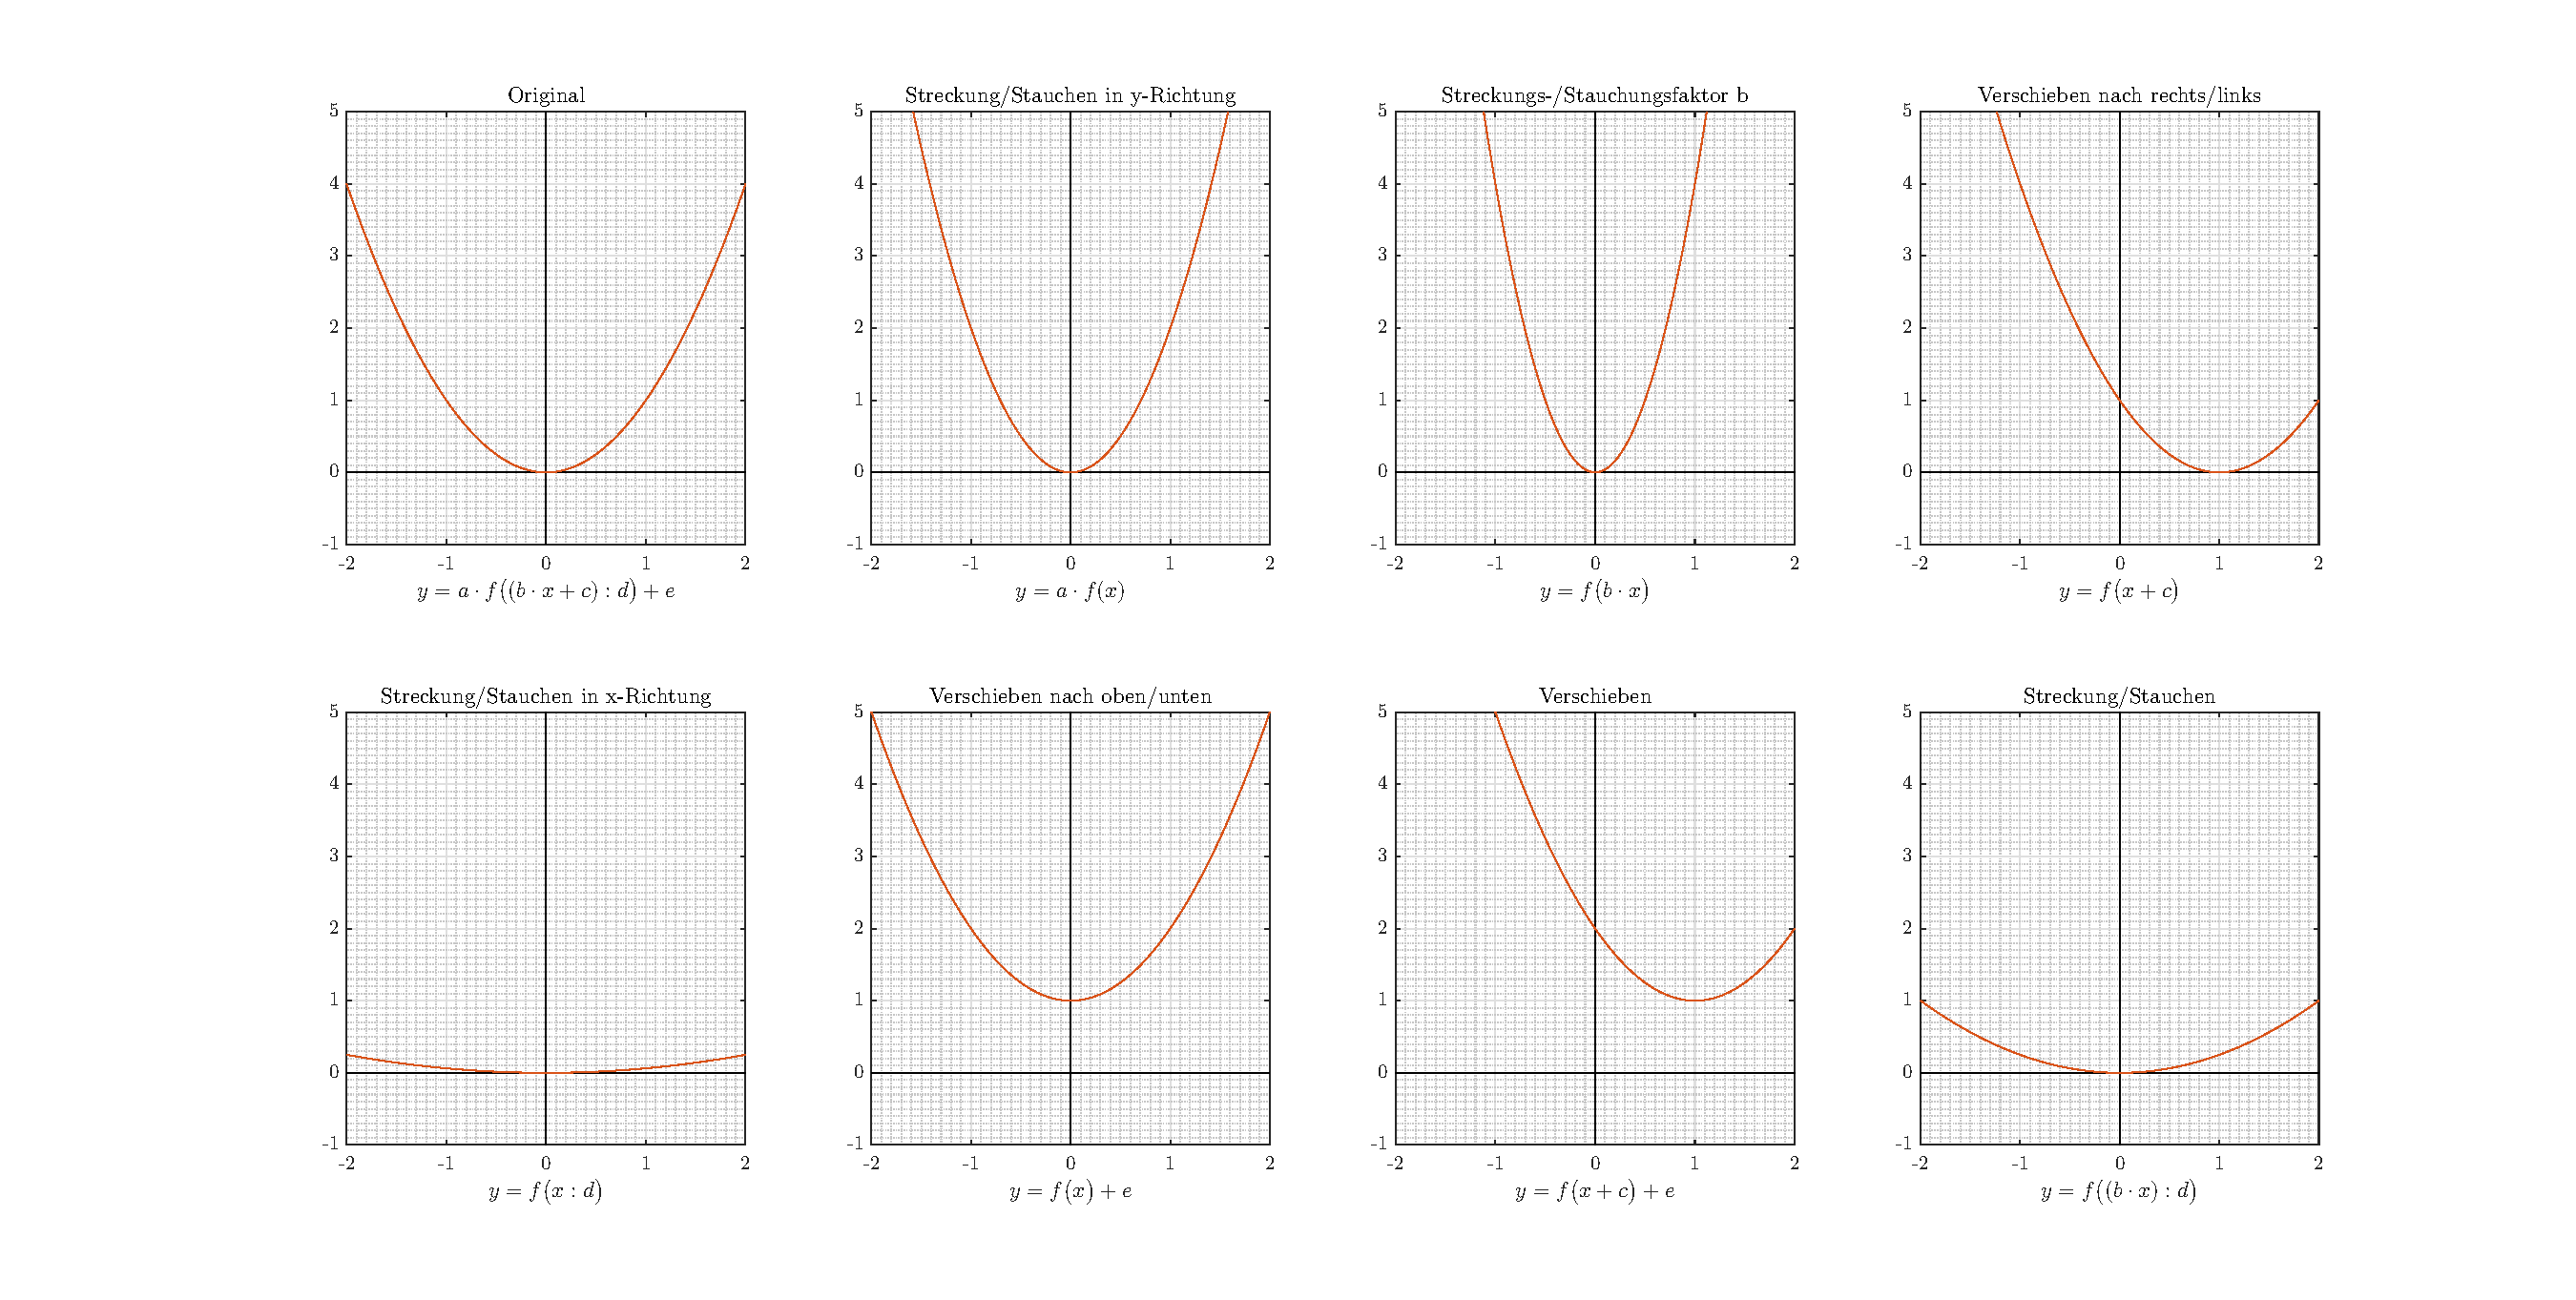
\includegraphics[height=20cm,trim={5cm 1cm 22cm 1cm},clip]{fig.eps}
		}
	\end{sidewaysfigure}
	\begin{sidewaysfigure}
		\centering
		\fbox{
			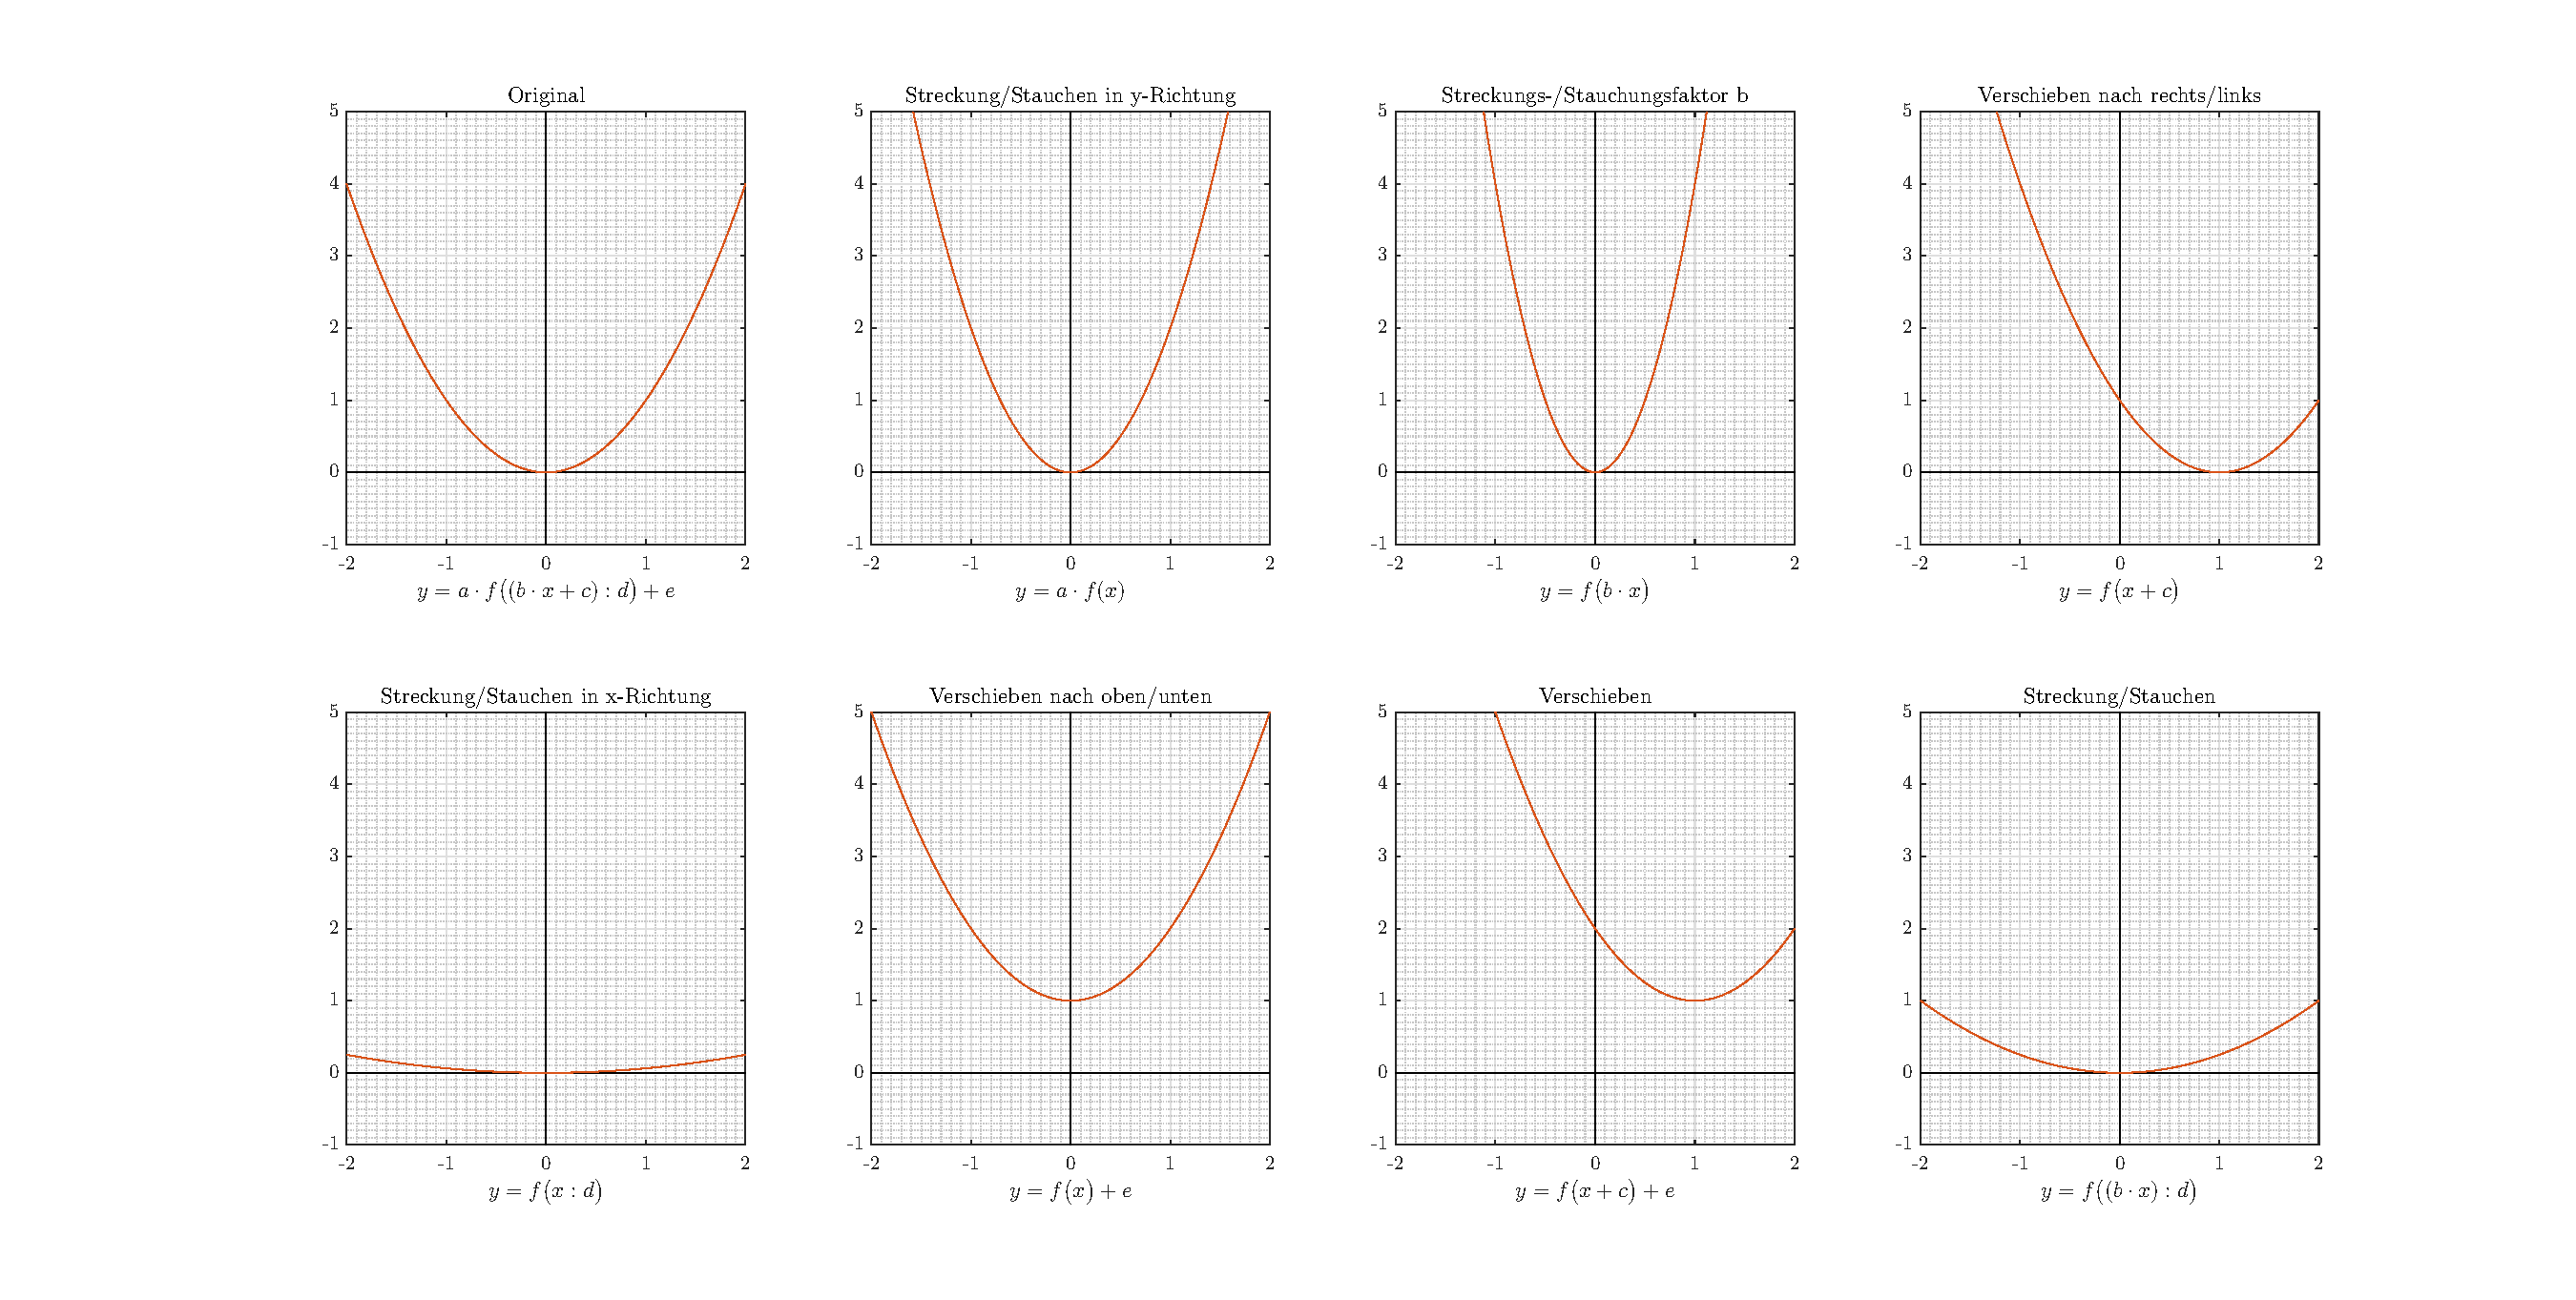
\includegraphics[height=20cm,trim={23cm 1cm 3cm 1cm},clip]{fig.eps}
		}
	\end{sidewaysfigure}
\end{document}